\label{chap:arch}
\subsection{Hardware}

The wireless sensor nodes use an Atmel ZigBit 900MHZ RF module, that contains an ATmega 1281v microcontroller connected with an AT86RF212 RF Tranceiver through a SPI interface. The module is a very low power device, capable of sending data up to 6 km. The Tranceiver contains a security module compatible with AES-128. It supports hardware encryption and decryption AES 128 ECB, but only hardware encryption AES 128 CBC.

\begin{figure}
  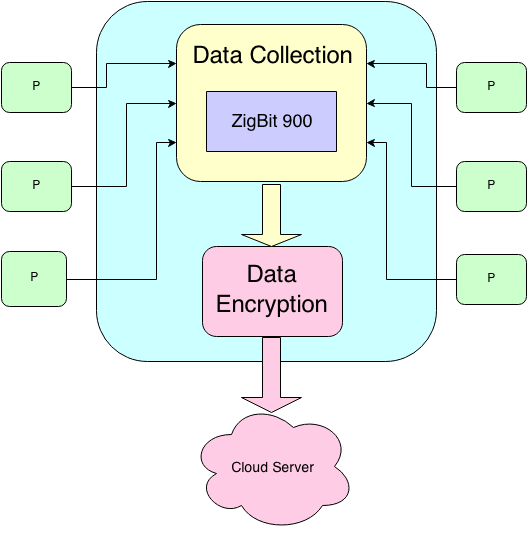
\includegraphics[width=0.5\textwidth]{wsn_soa_system_arch}
\end{figure}

\section{Software}

From the software perspective, the architecture is composed of two parts: gathering data from the sensors and encrypting it before transmitting it to another sensor of the central gateway.
The encryption method for the data shall use both of the hardware supported methods: AES 128 ECB and AES 128 CBC. It is necessary to use them both because the nodes shall be transmitiing 
two kinds of packets: a first set which contains non-sensitive data and is used by the receiver to identify the sender and a second which contains the actual sensitive data. Since it supports 
both encryption and decryption, the first set of packets, those containing identification information, shall be encrypted using ECB. The data itself shall be encrypted using CBC. Since CBC 
decryption is not supported by default, a software CBC decryption implementation is necessary in order to allow the sensors to verify the data at regular intervals.

\begin{figure}
  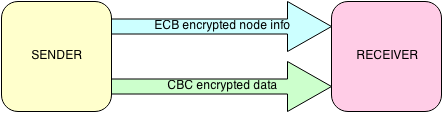
\includegraphics[width=0.5\textwidth]{send_receive}
\end{figure}

In addition to the CBC decryption, it is also required to have implementations of other software encryption algorithms in order to perform the performance analysis. The chosen 
algorithms which shall be used in benchmarking are Skipjack and RC5.
